% !TeX spellcheck = en_GB
\section{Dynamic Tropopause map}
\label{sec:DT}
The dynamic tropopause map (DT), shown in \Cref{fig:DynTropo} presents the potential temperature distribution at the tropopause. Colder tropopause is associated with colder colours and vice versa warmer tropopause with warmer colours (shading according to the colorbar). Therefore, a warmer tropopause indicates an elevation of the atmospheric column. 
\\
The gradient at the \SI{2}{PVU} (\SI{1}{PV} unit = \SI{e-6}{\metre\squared\per\s\kelvin\per\kg}; \cite{hoskins_use_1985}) surface, between the cold and warm area indicates the thermal wind. There is a slope between the cold and warm surfaces increasing towards the warmer column averaged temperature. An increased slope means also an increased pressure gradient force with increasing height and therefore an increase in geostrophic wind. This means, that there exists a vertical wind shear. From this, the mid-latitude jet stream can be pointed out.  \textcolor{red}{do I need to present the equation of thermal wind?} Wind barbs in \SI{}{\mPs} indicate the direction of the wind flow, which is generally from west to east in the mid-latitudes.  
\\
The  \SI{925}-\SI{850}{\hPa} layer-averaged surface relative vorticity is shown in black contours, every \SI{.5e-4}{\per\second}. It represents the rotation of a fluid. \textcolor{red}{Does the relative vorticity need more explanation? }
\\
Along the Rossby-Wave-Guide, troughs and ridges are seen which can be combined with the surface relative vorticity to understand the vertical dynamic interaction in the atmosphere. In case of a westward tilt between the surface cyclone and an upper level through an intensification of the surface cyclone is more likely to occur.

%%% Dynamic tropopause map %%%%%%%%%%%%%%%%%%%%%%%%%%%%%%%%%%%%%
% !TeX spellcheck = en_GB
\begin{figure}[h!]
    \centering
%%%%%% 20/12
    \begin{subfigure}[b]{0.49\textwidth}
        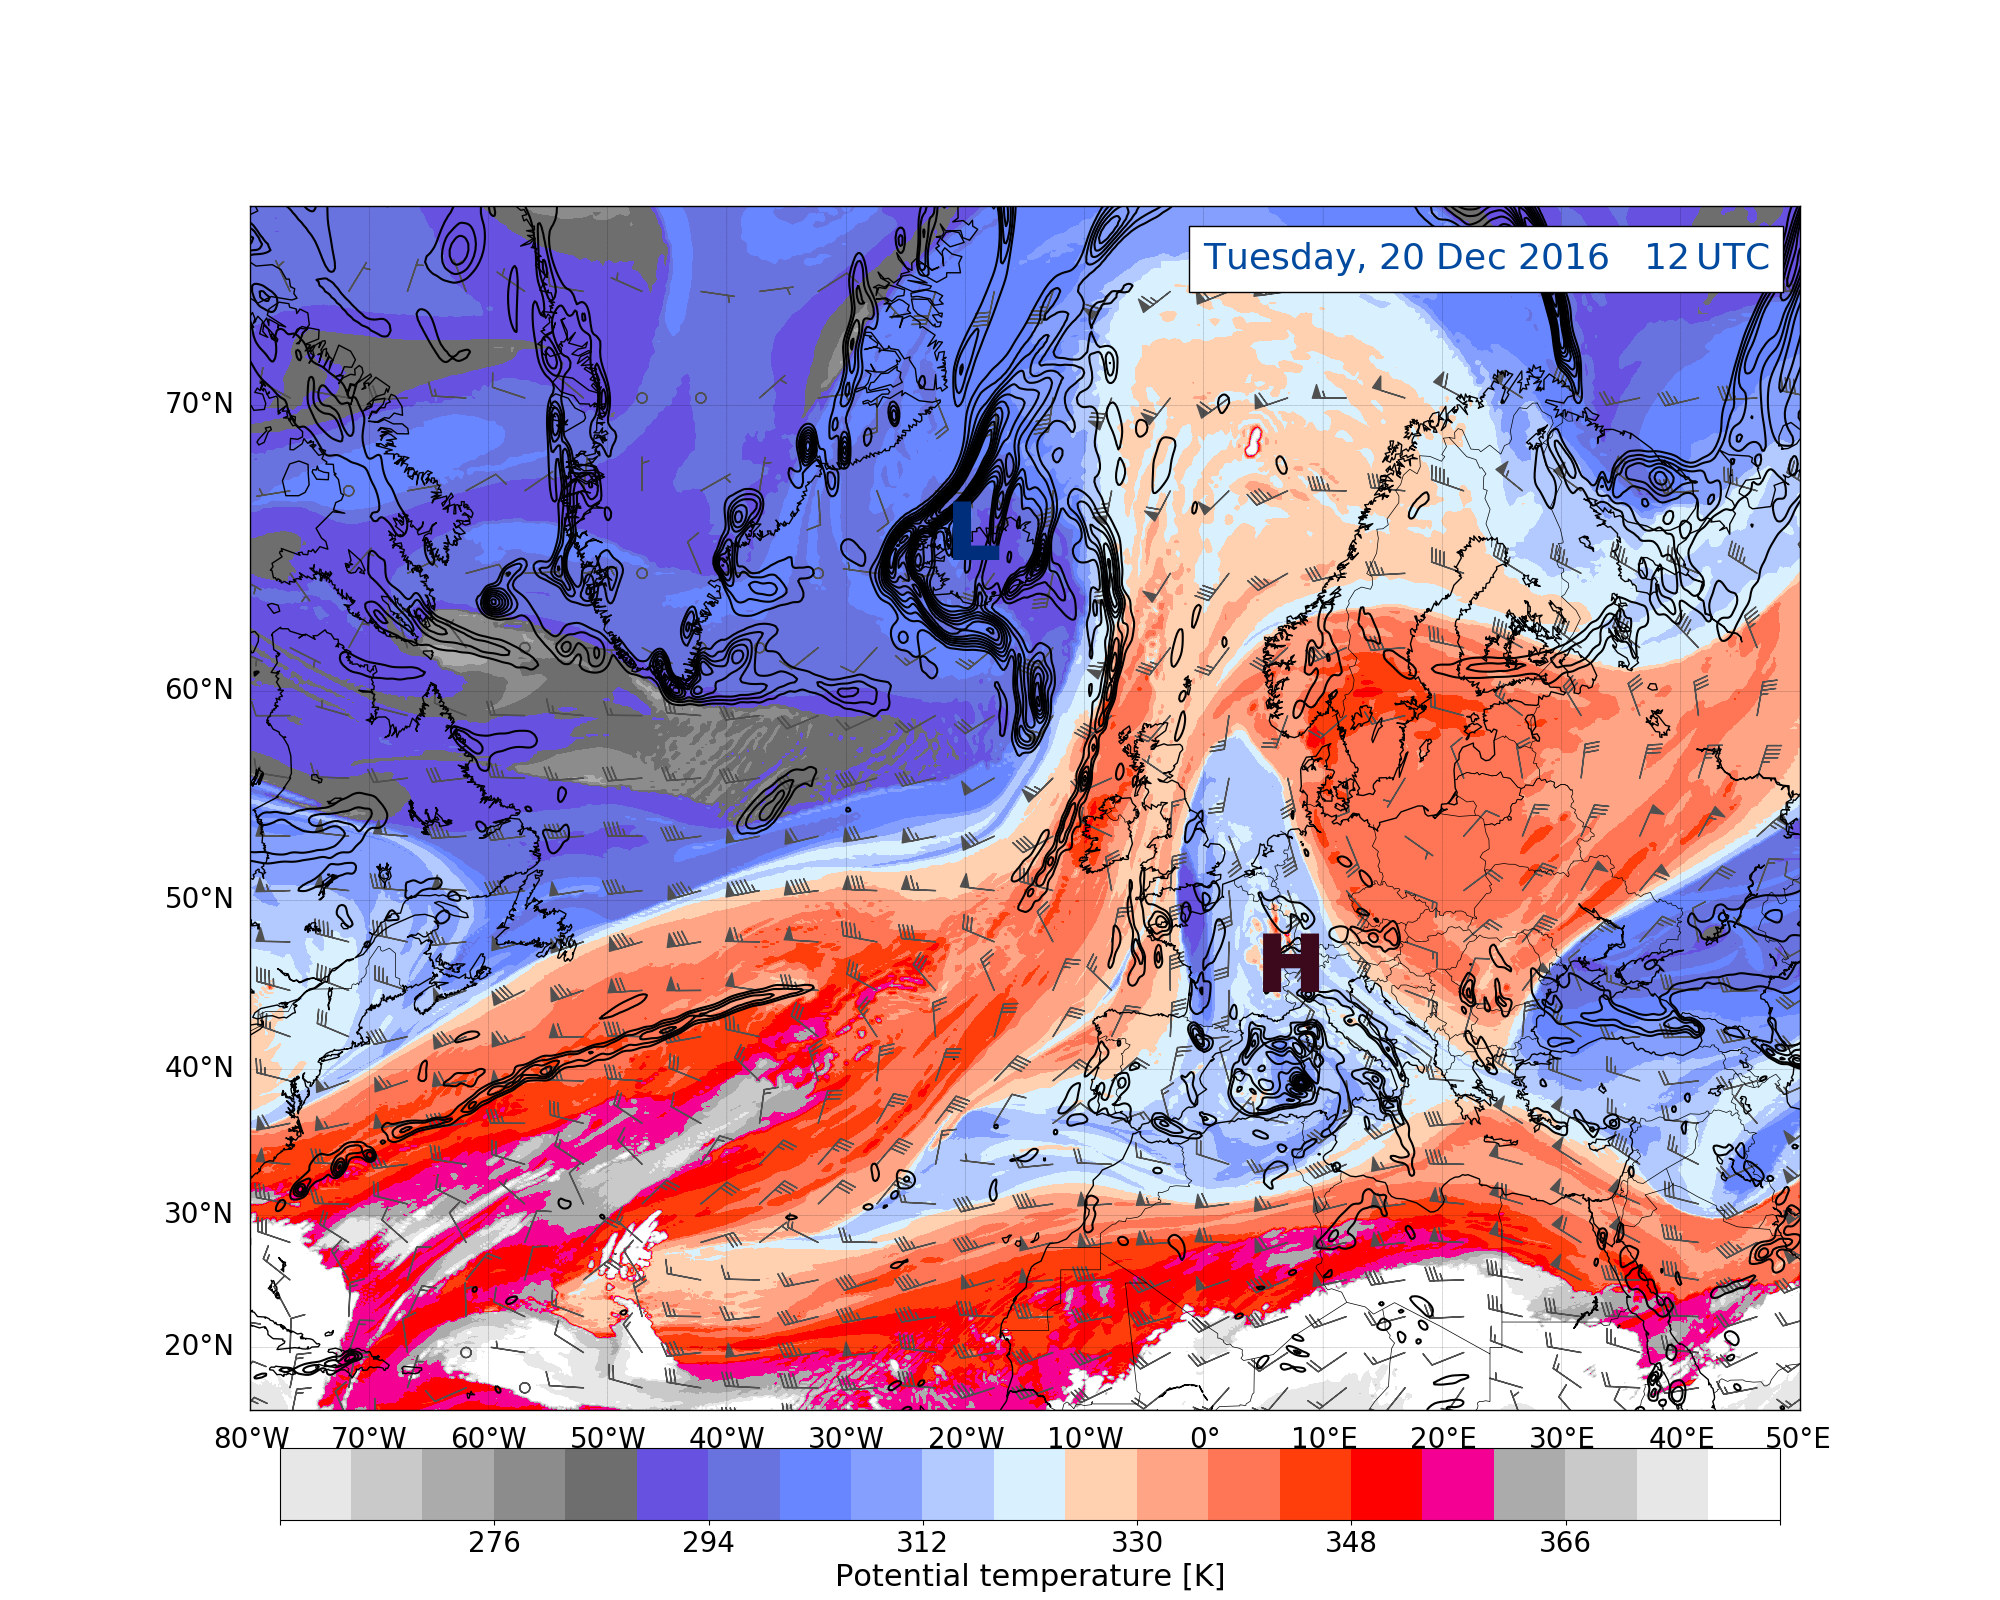
\includegraphics[trim={4.2cm 3.9cm 4.3cm 5.1cm},clip,
        width=\textwidth]{./fig_DynTropo/20161220_12}
        \caption{} \label{fig:DT20}
    \end{subfigure}
%%%%%% 21/12
    \begin{subfigure}[b]{0.49\textwidth}
        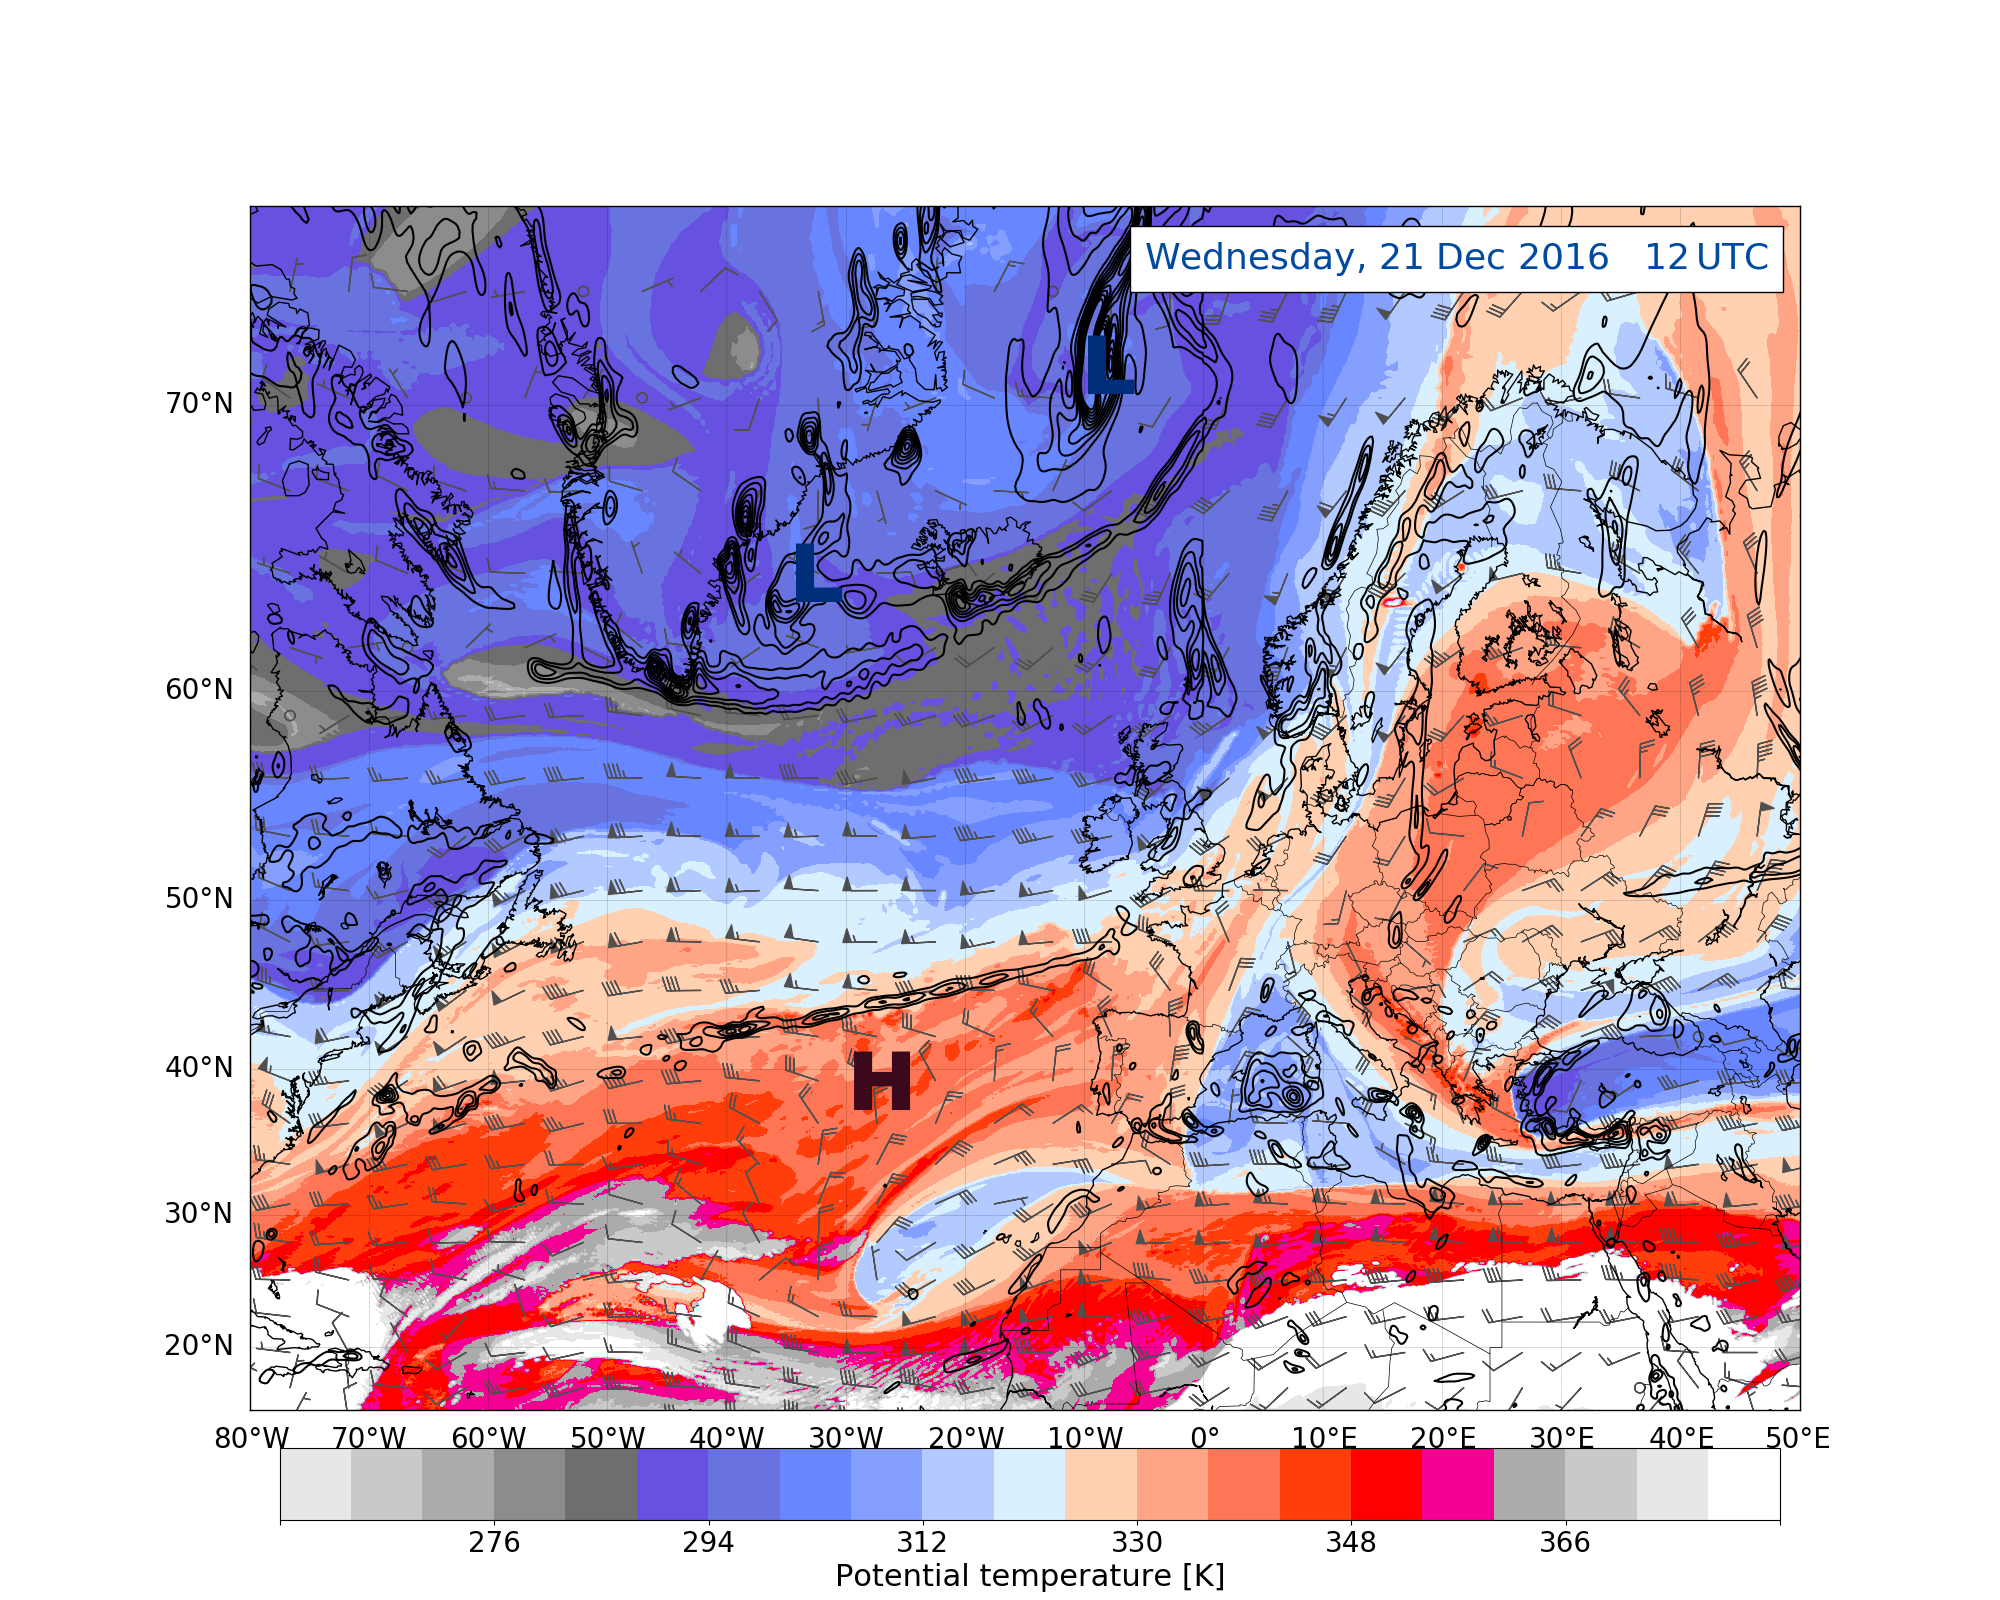
\includegraphics[trim={4.2cm 3.9cm 4.3cm 5.1cm},clip,
        width=\textwidth]{./fig_DynTropo/20161221_12}
        \caption{}\label{fig:DT21}
    \end{subfigure}

%%%%%% 22/12
\begin{subfigure}[b]{0.49\textwidth}
	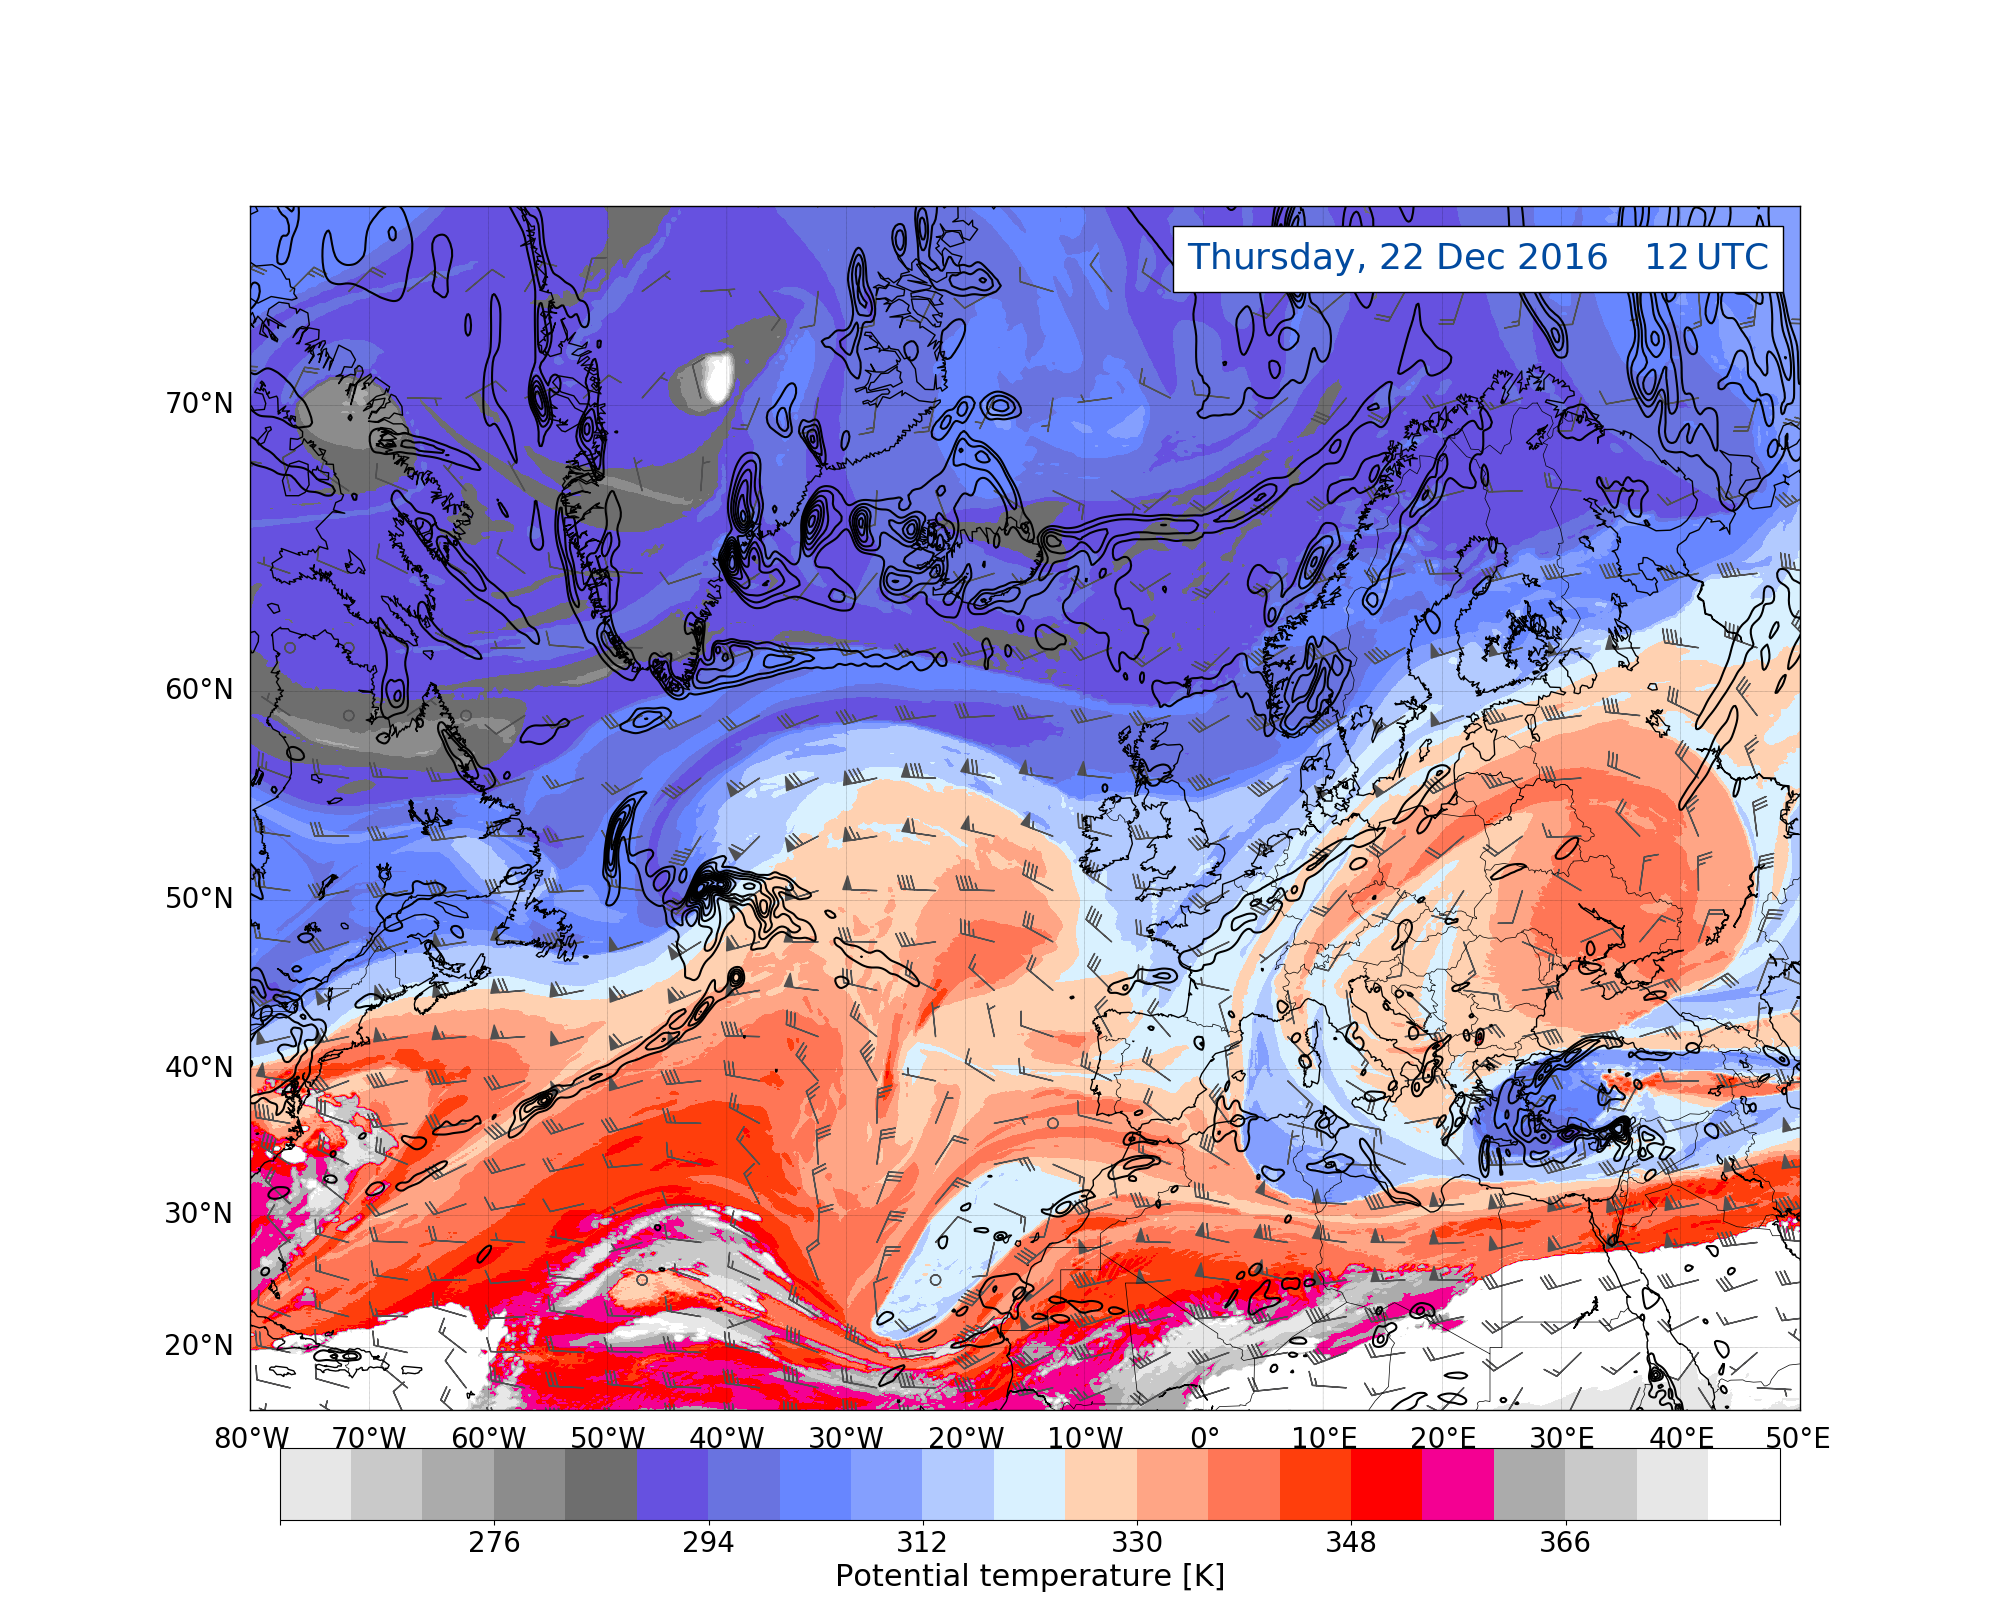
\includegraphics[trim={4.2cm 3.9cm 4.3cm 5.1cm},clip,
	width=\textwidth]{./fig_DynTropo/20161222_12}
	\caption{}\label{fig:DT22}
\end{subfigure}
%%%%%% 23/12
\begin{subfigure}[b]{0.49\textwidth}
	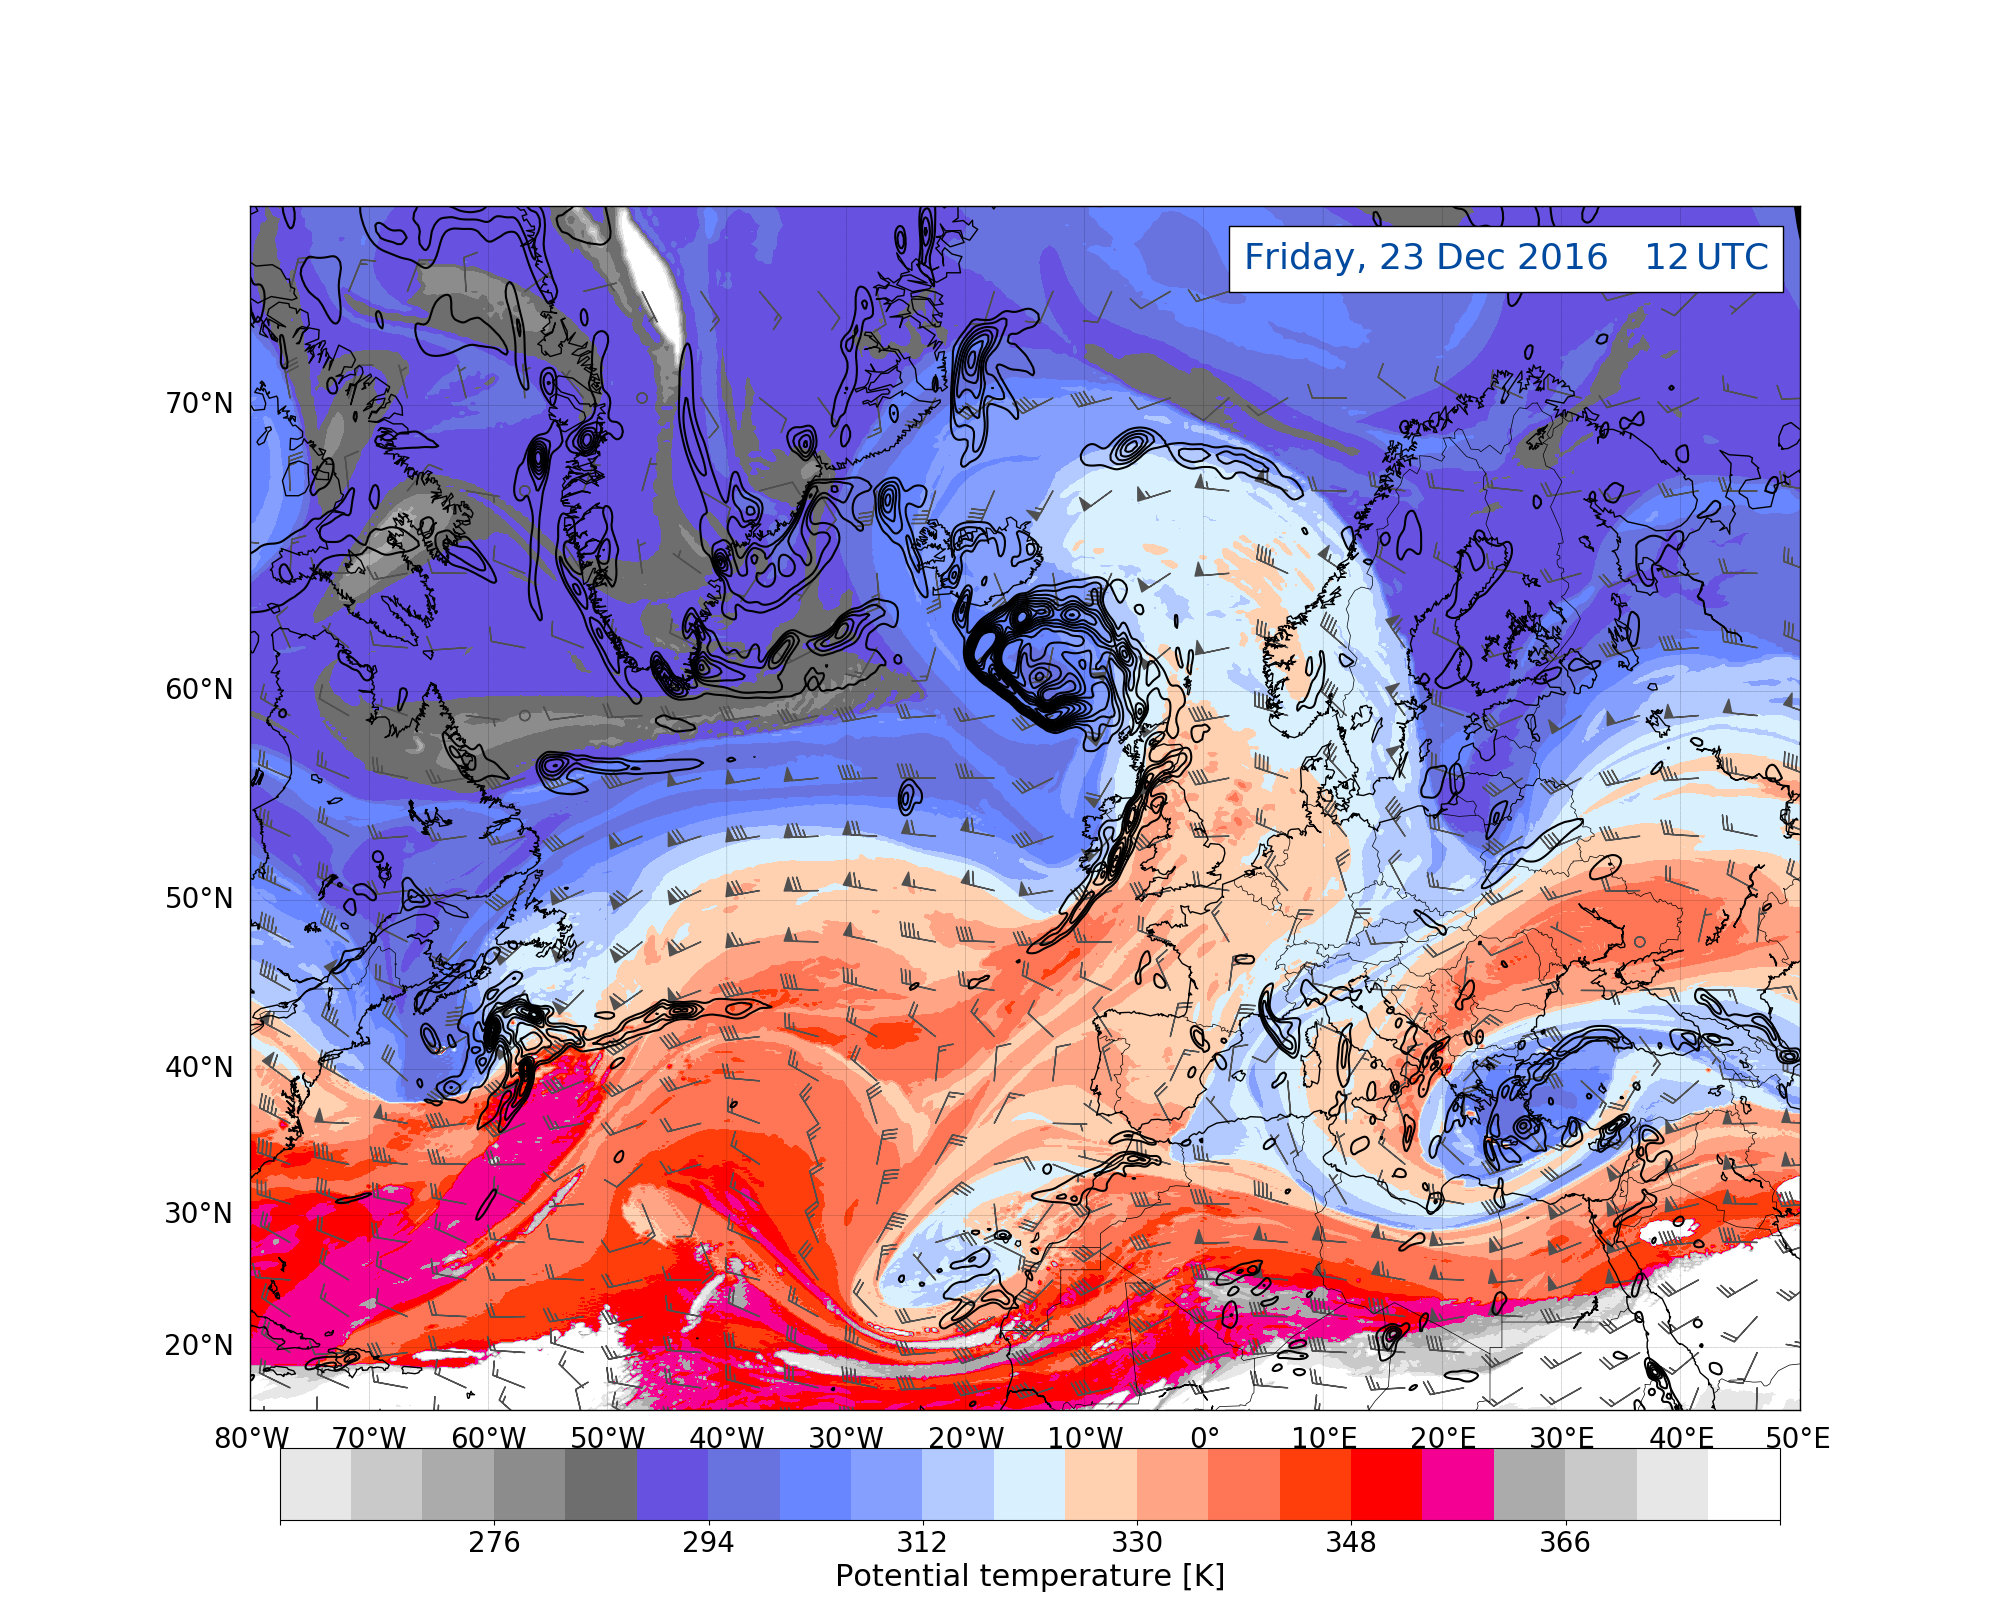
\includegraphics[trim={4.2cm 3.9cm 4.3cm 5.1cm},clip,
	width=\textwidth]{./fig_DynTropo/20161223_12}
	\caption{}\label{fig:DT23}
\end{subfigure}

%%%%%% label
    \begin{subfigure}[b]{\textwidth}
        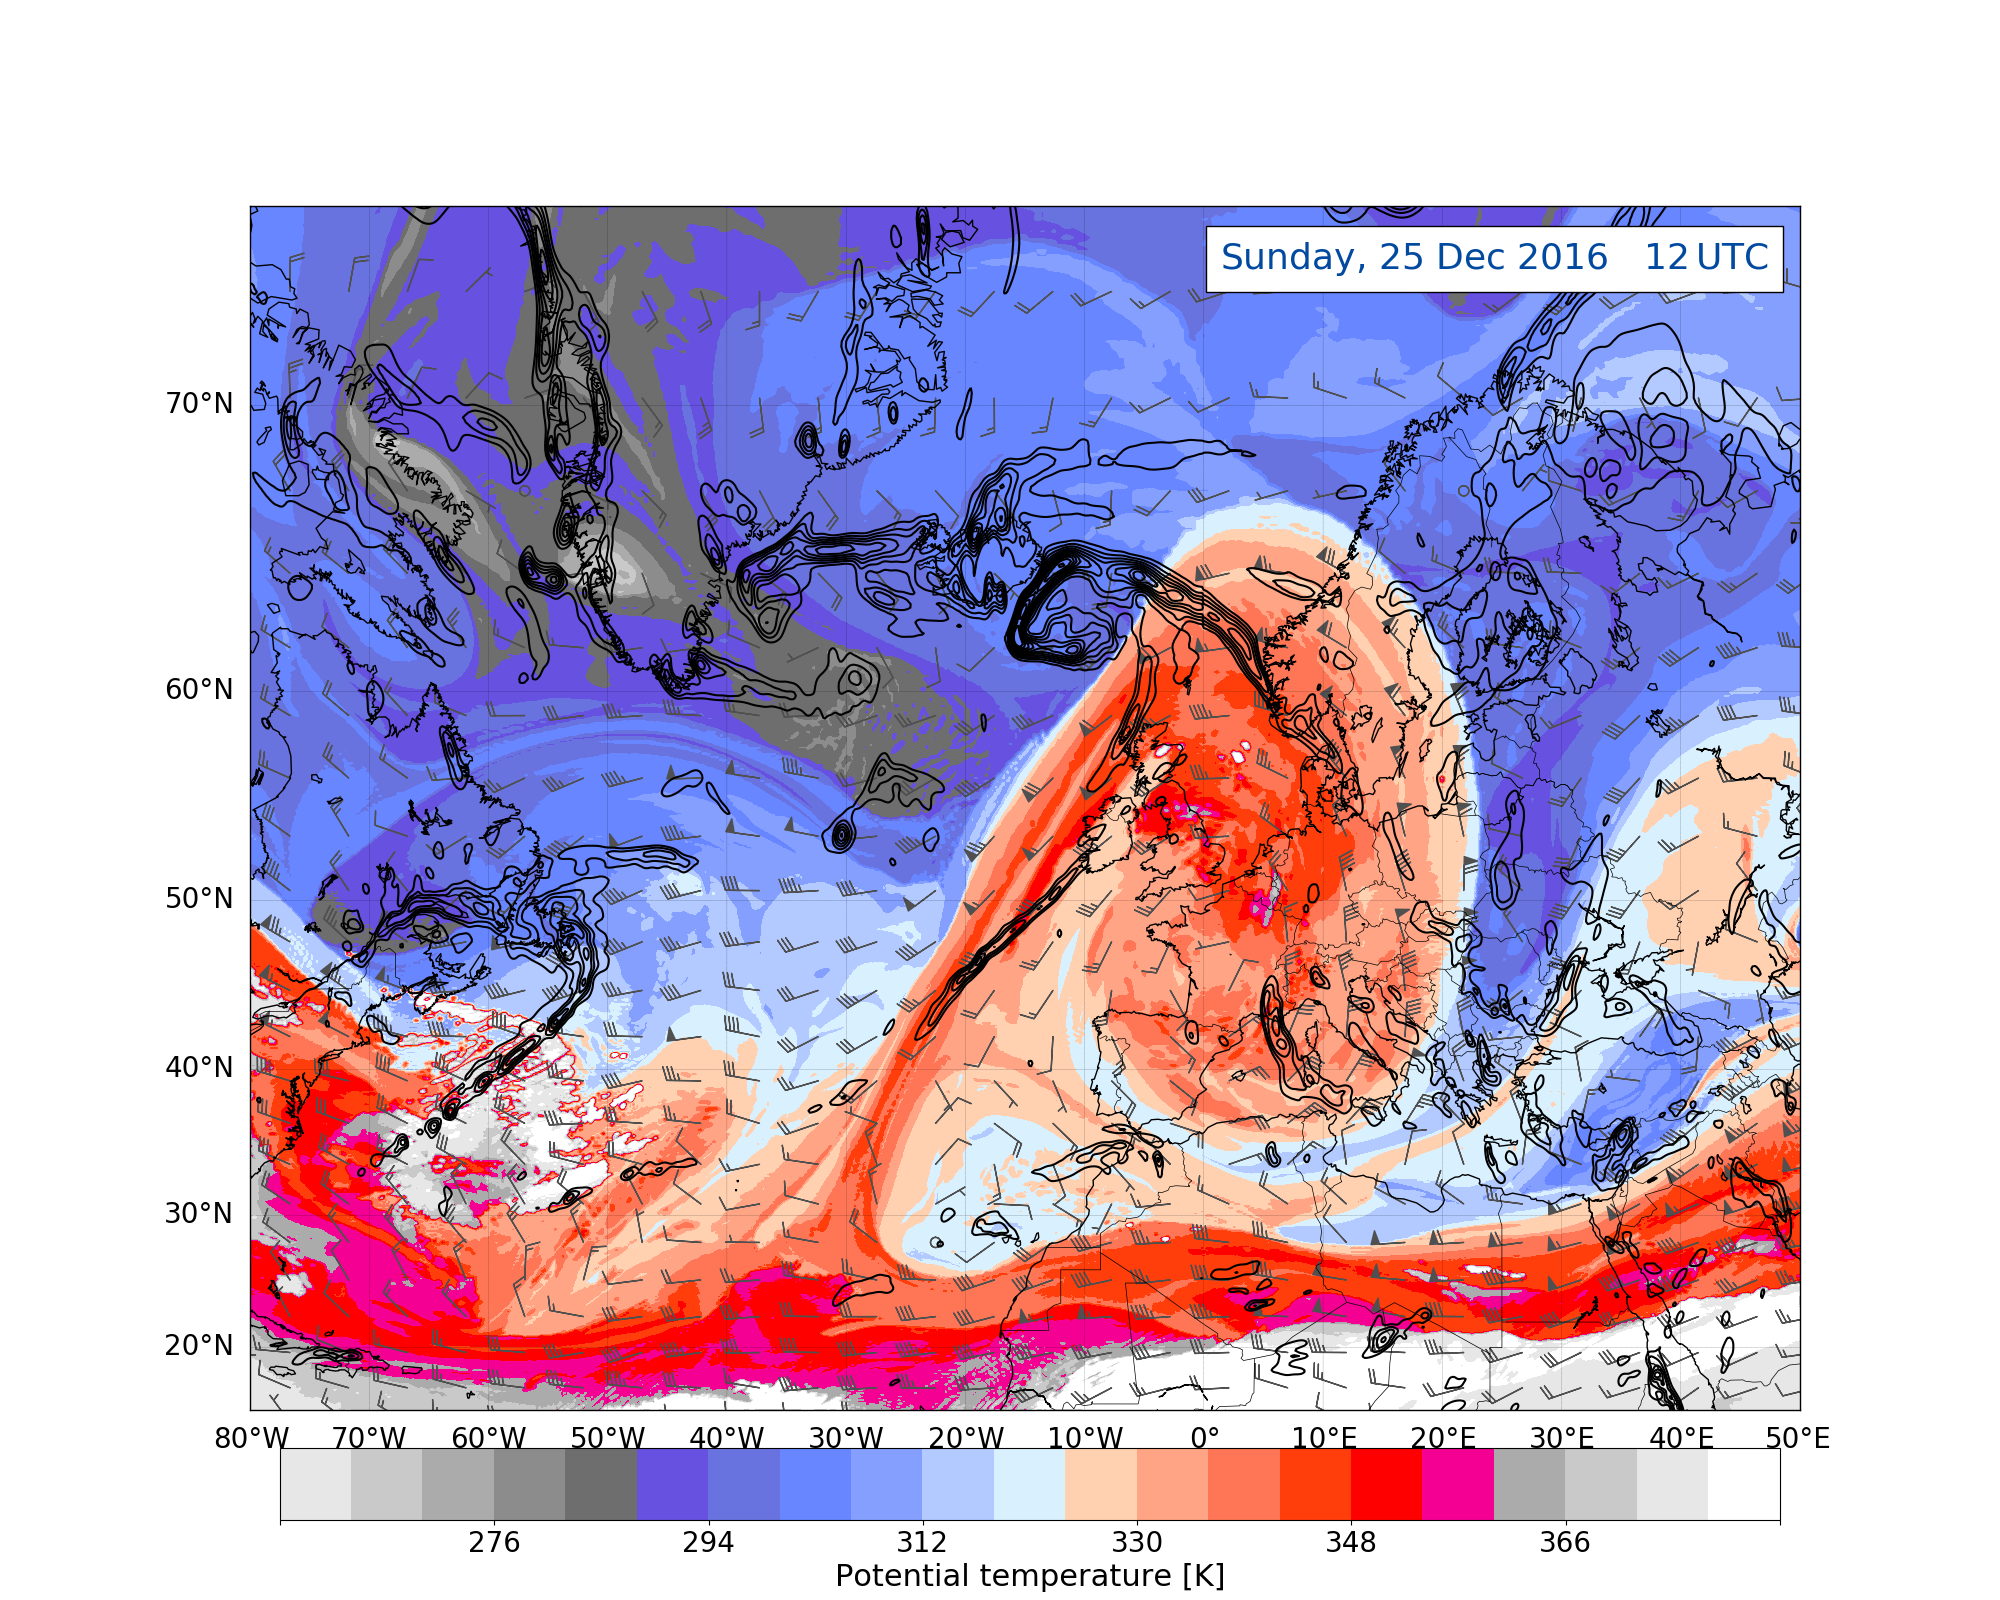
\includegraphics[trim={4.2cm 0cm 4.3cm 36.8cm},clip,
        width=\textwidth]{./fig_DynTropo/20161225_12}
    \end{subfigure}
\end{figure}
%
\begin{figure}\ContinuedFloat
	\centering
%%%%%% 24/12
    \begin{subfigure}[b]{0.49\textwidth}
        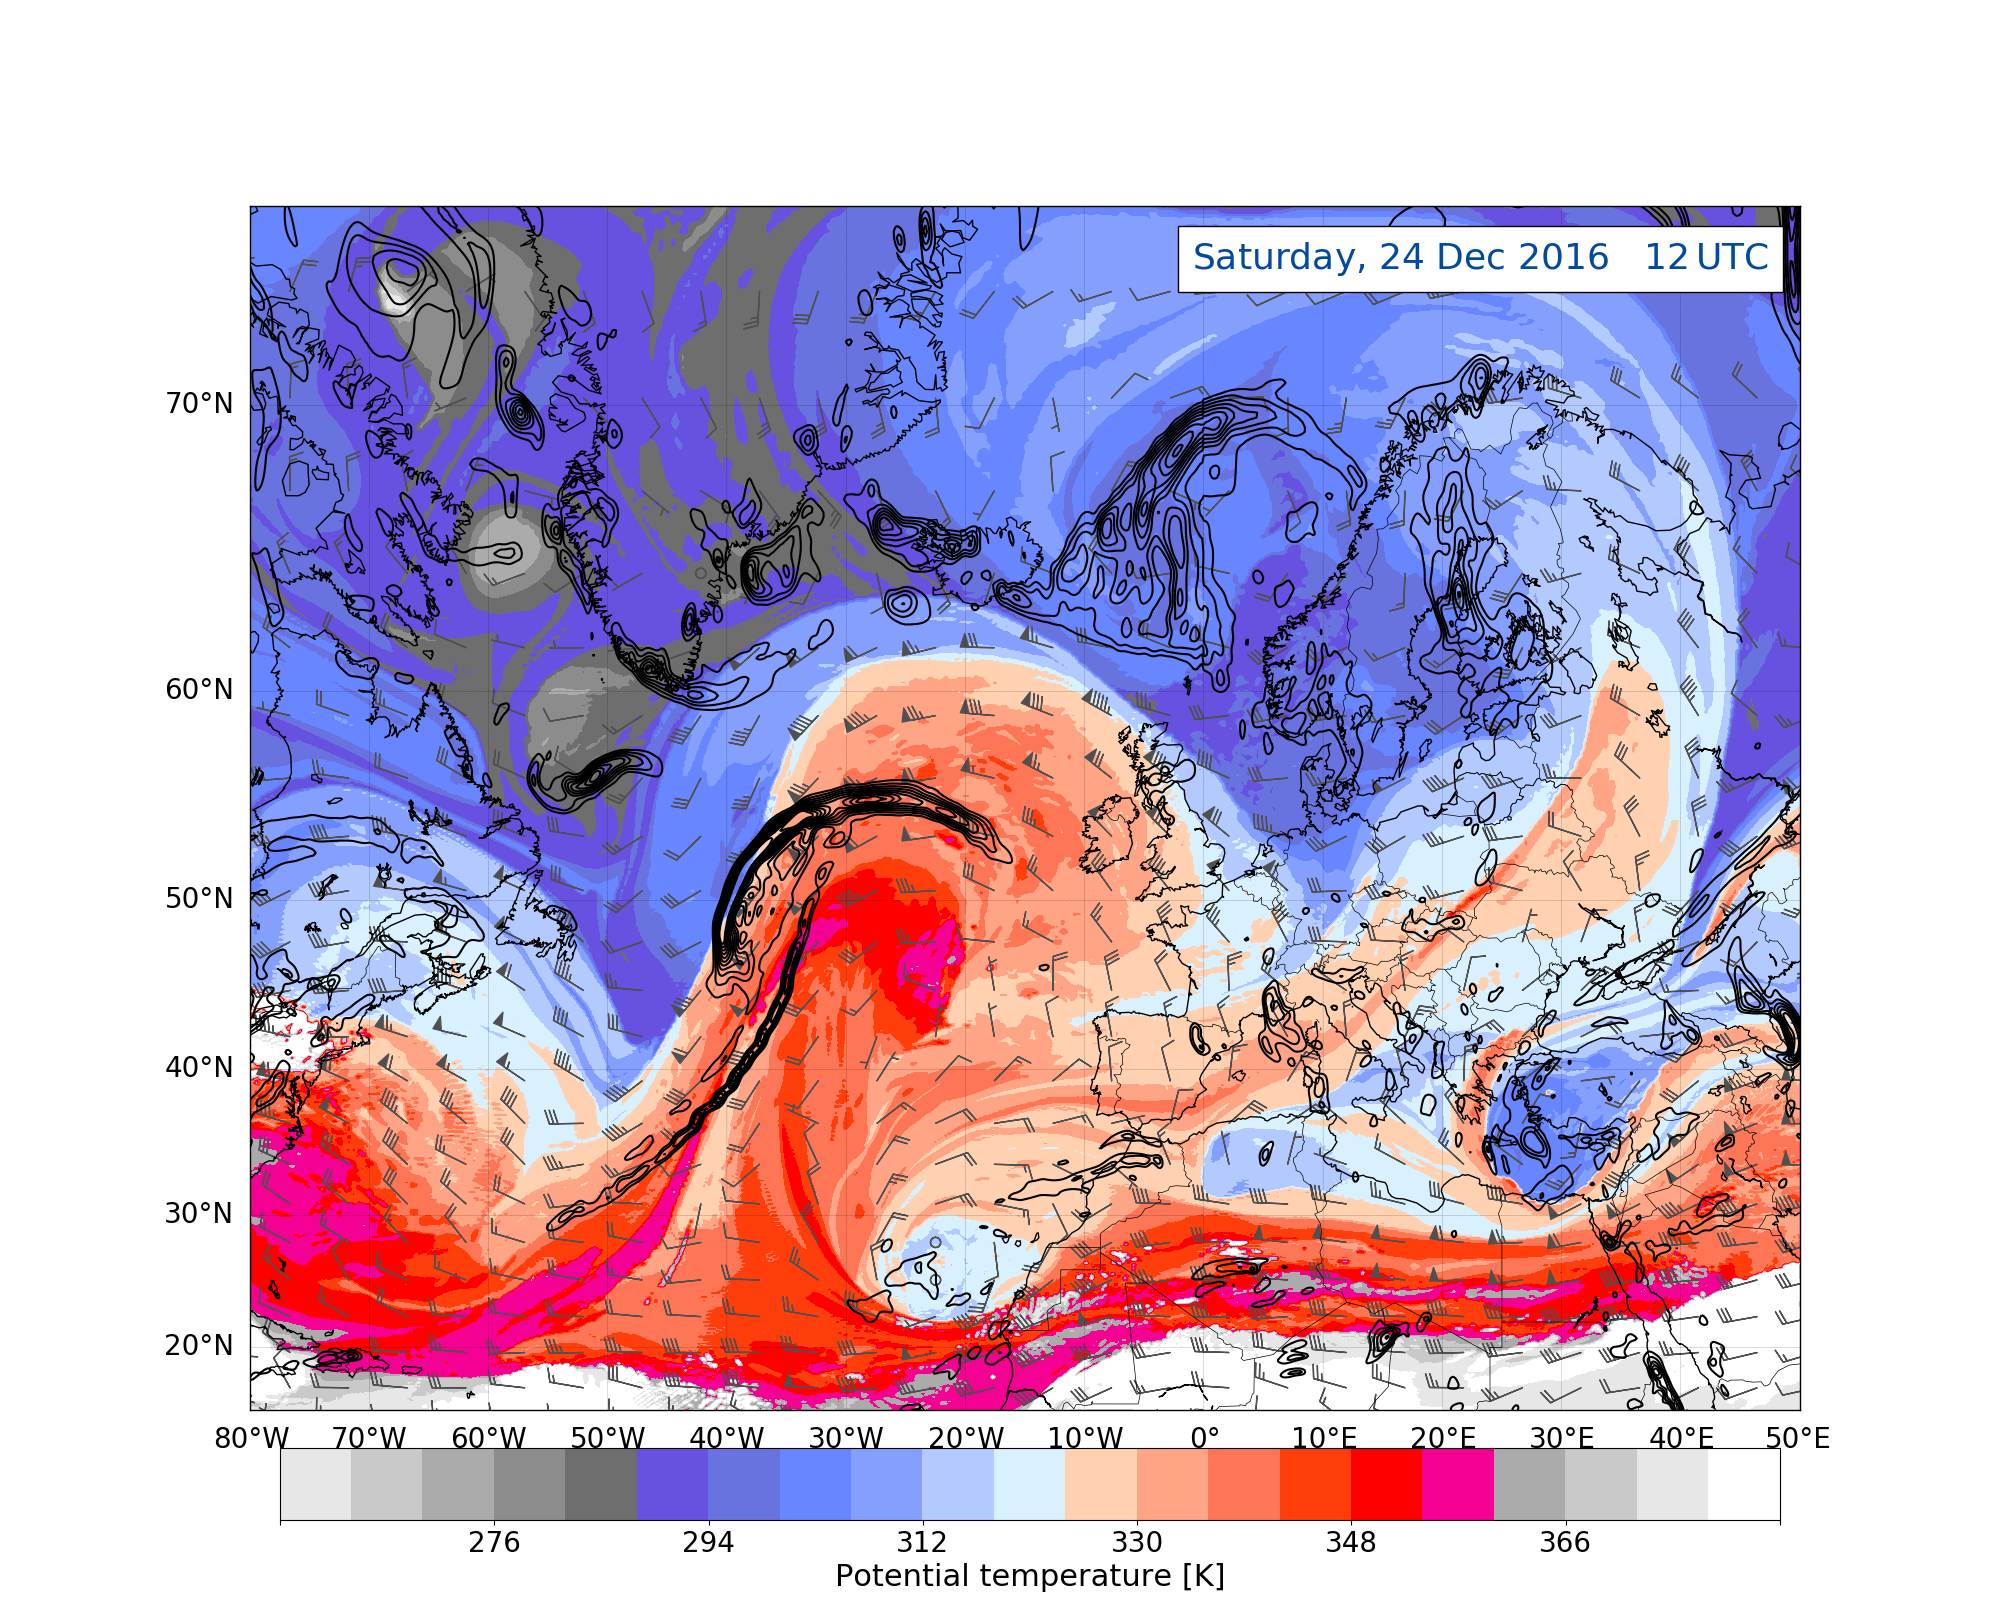
\includegraphics[trim={4.2cm 3.9cm 4.3cm 5.1cm},clip,
        width=\textwidth]{./fig_DynTropo/20161224_12}
        \caption{}\label{fig:DT24}
    \end{subfigure}
%%%%%% 25/12
    \begin{subfigure}[b]{0.49\textwidth}
        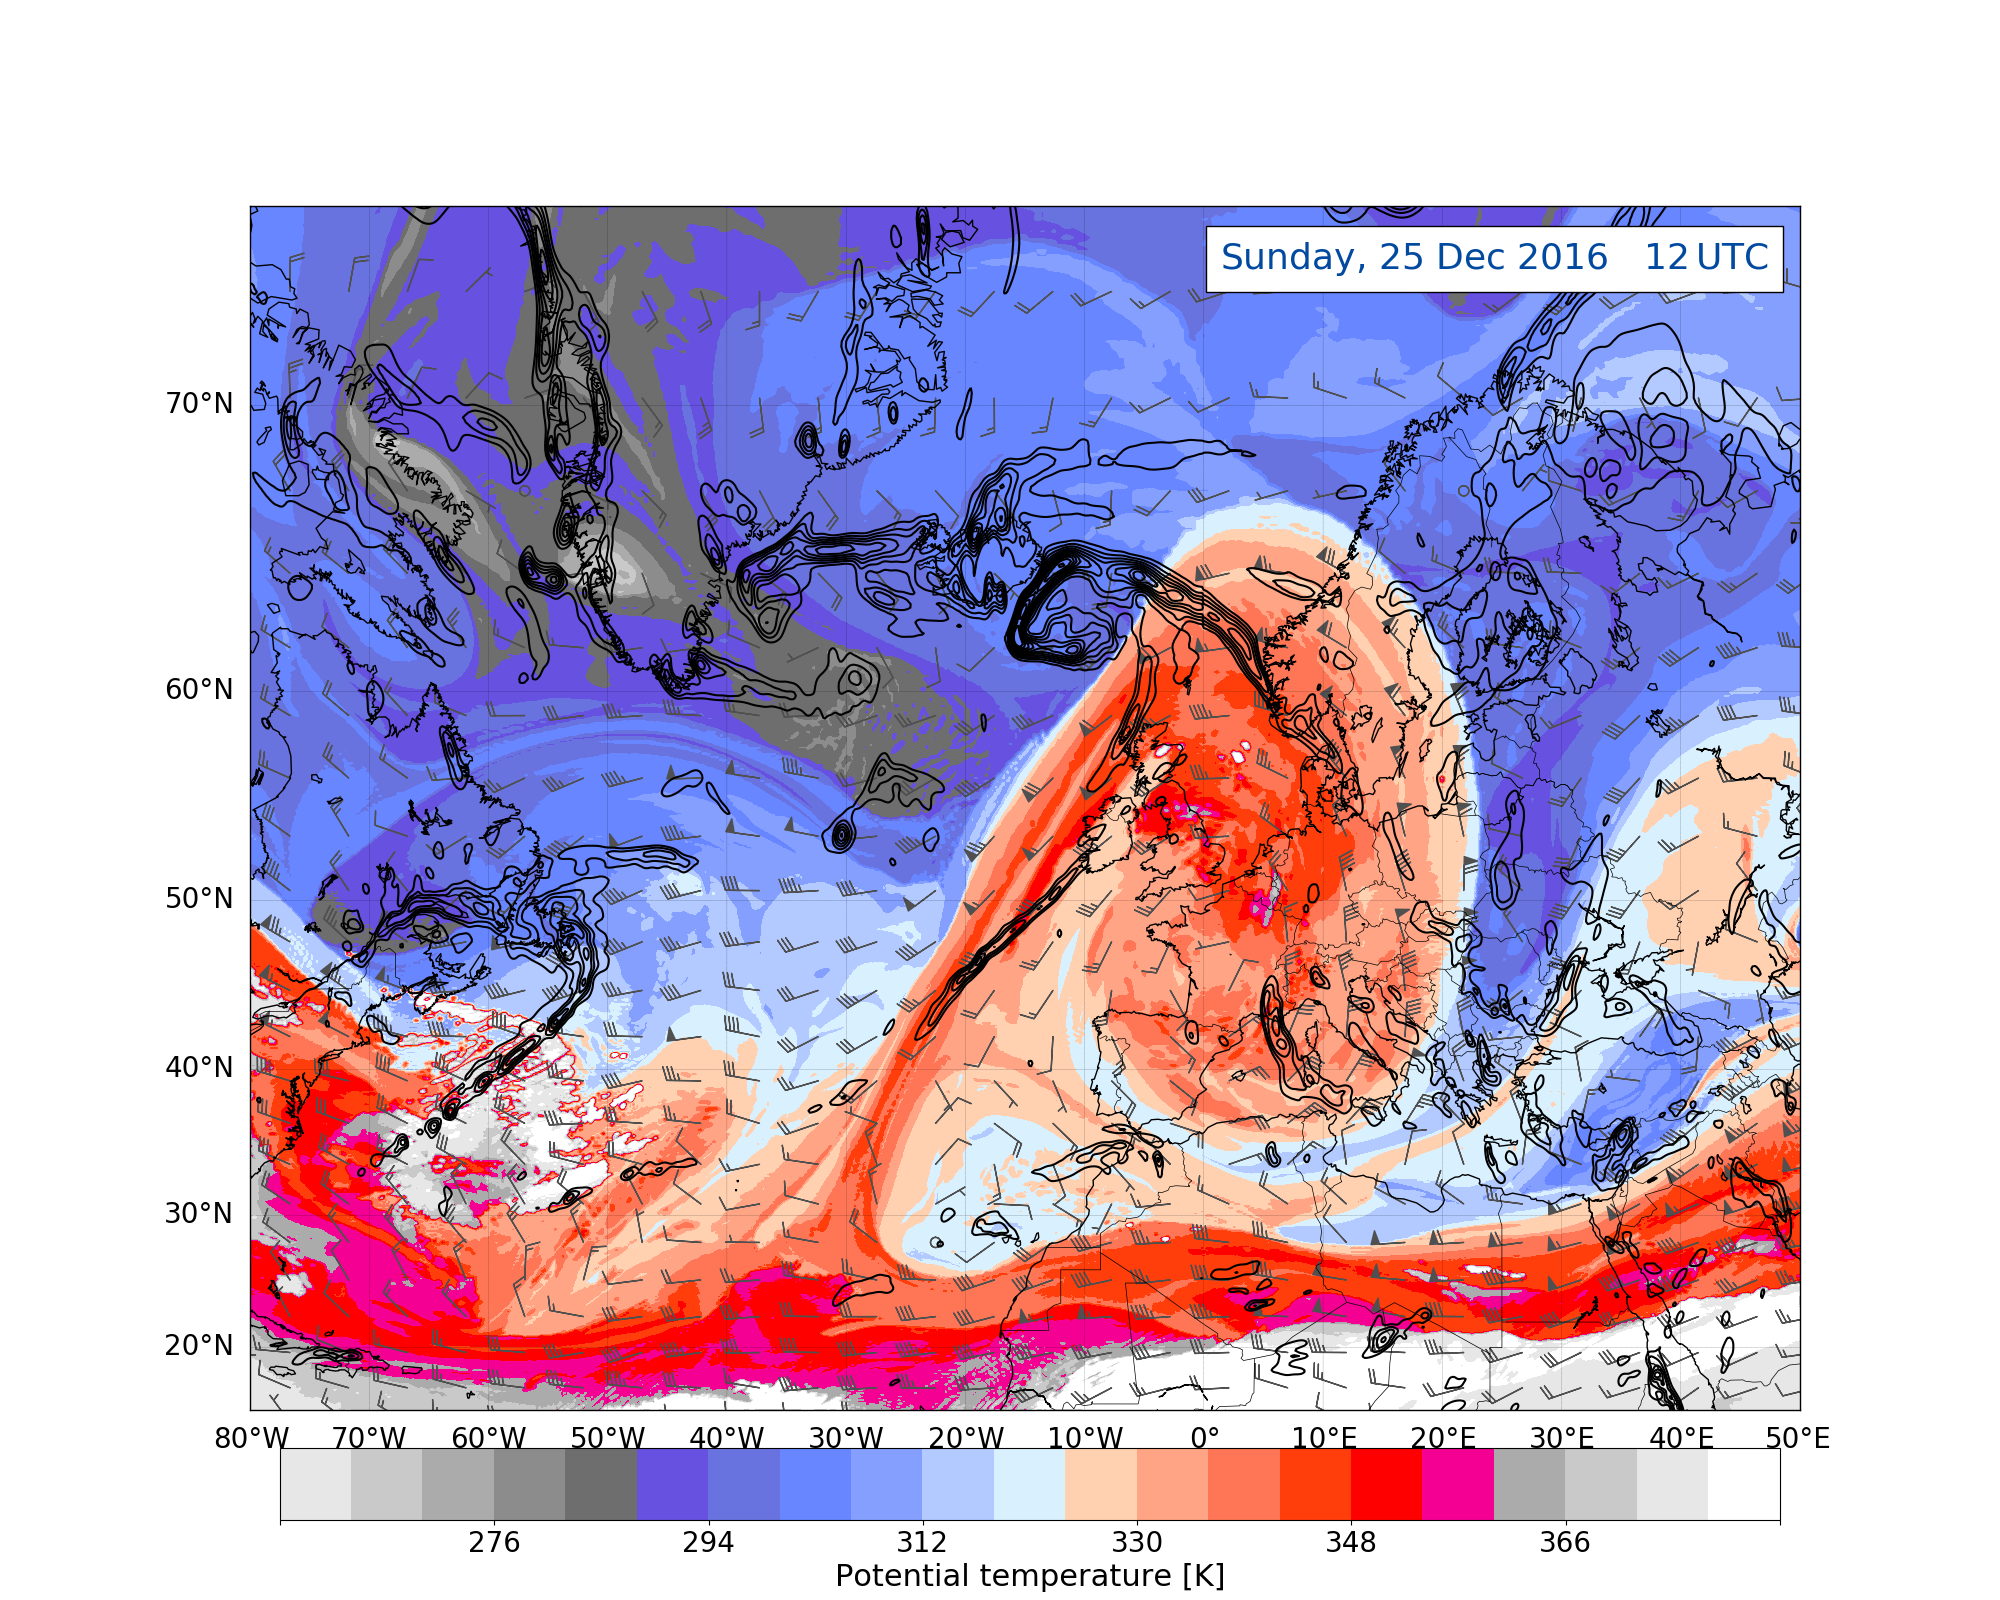
\includegraphics[trim={4.2cm 3.9cm 4.3cm 5.1cm},clip,
        width=\textwidth]{./fig_DynTropo/20161225_12}
        \caption{}\label{fig:DT25}
    \end{subfigure}    
%%%%%% 26/12
    \begin{subfigure}[b]{0.49\textwidth}
        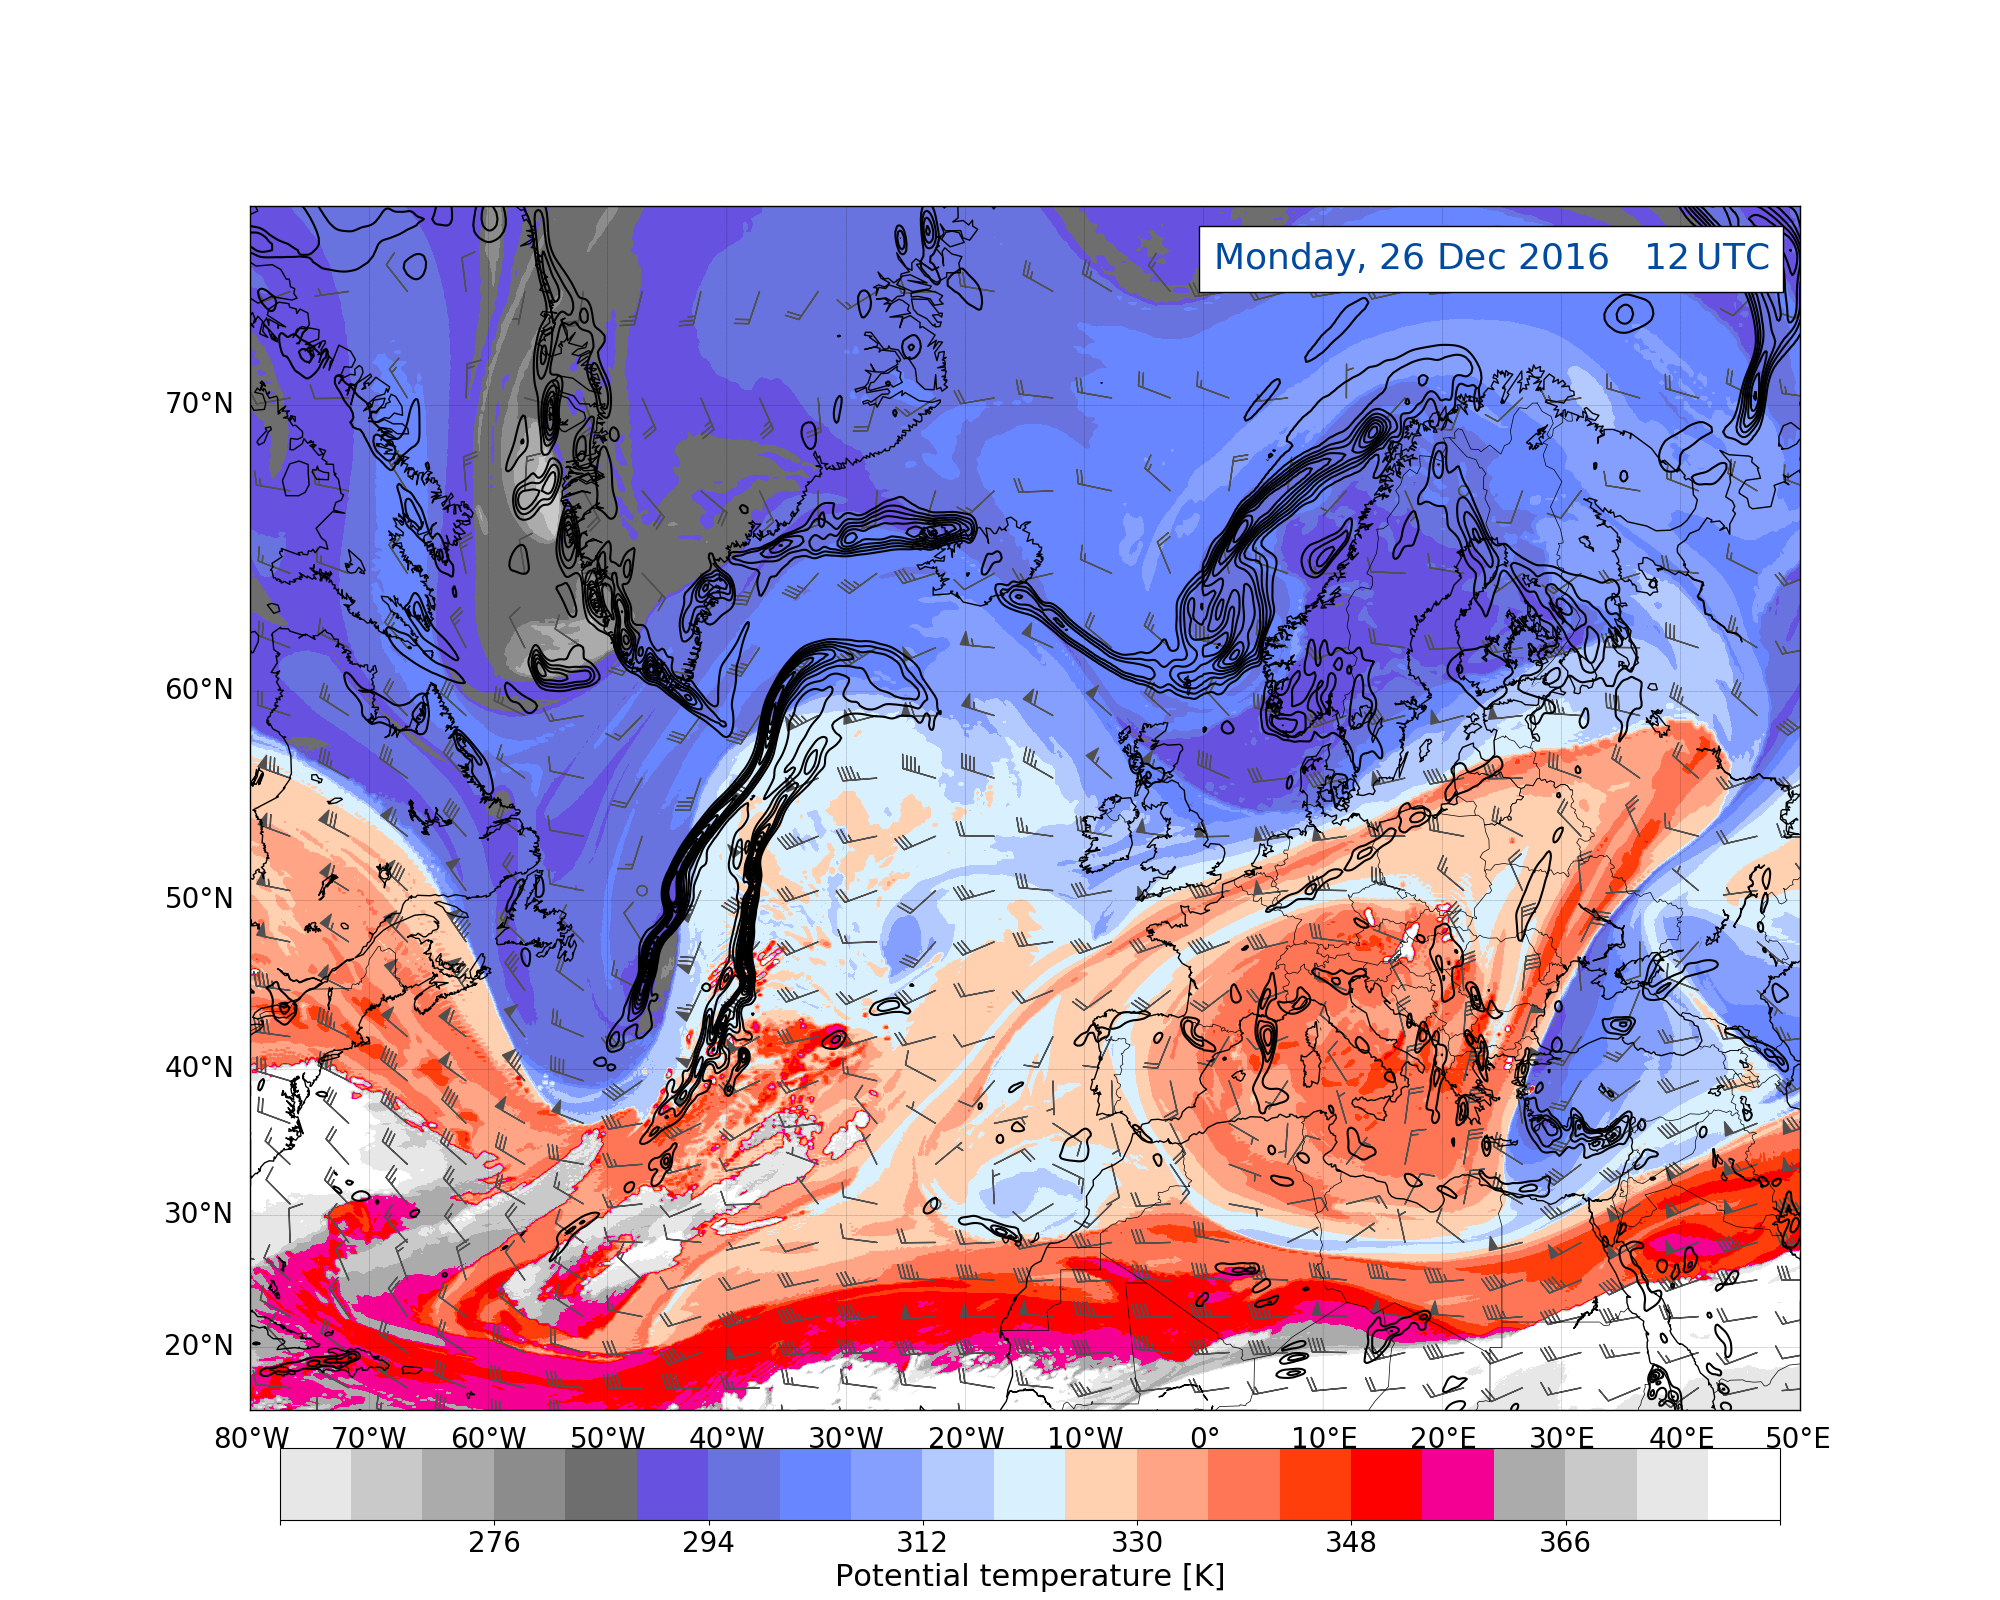
\includegraphics[trim={4.2cm 3.9cm 4.3cm 5.1cm},clip,
        width=\textwidth]{./fig_DynTropo/20161226_12}
        \caption{}\label{fig:DT26}
    \end{subfigure}
%%%%%% 27/12
    \begin{subfigure}[b]{0.49\textwidth}
        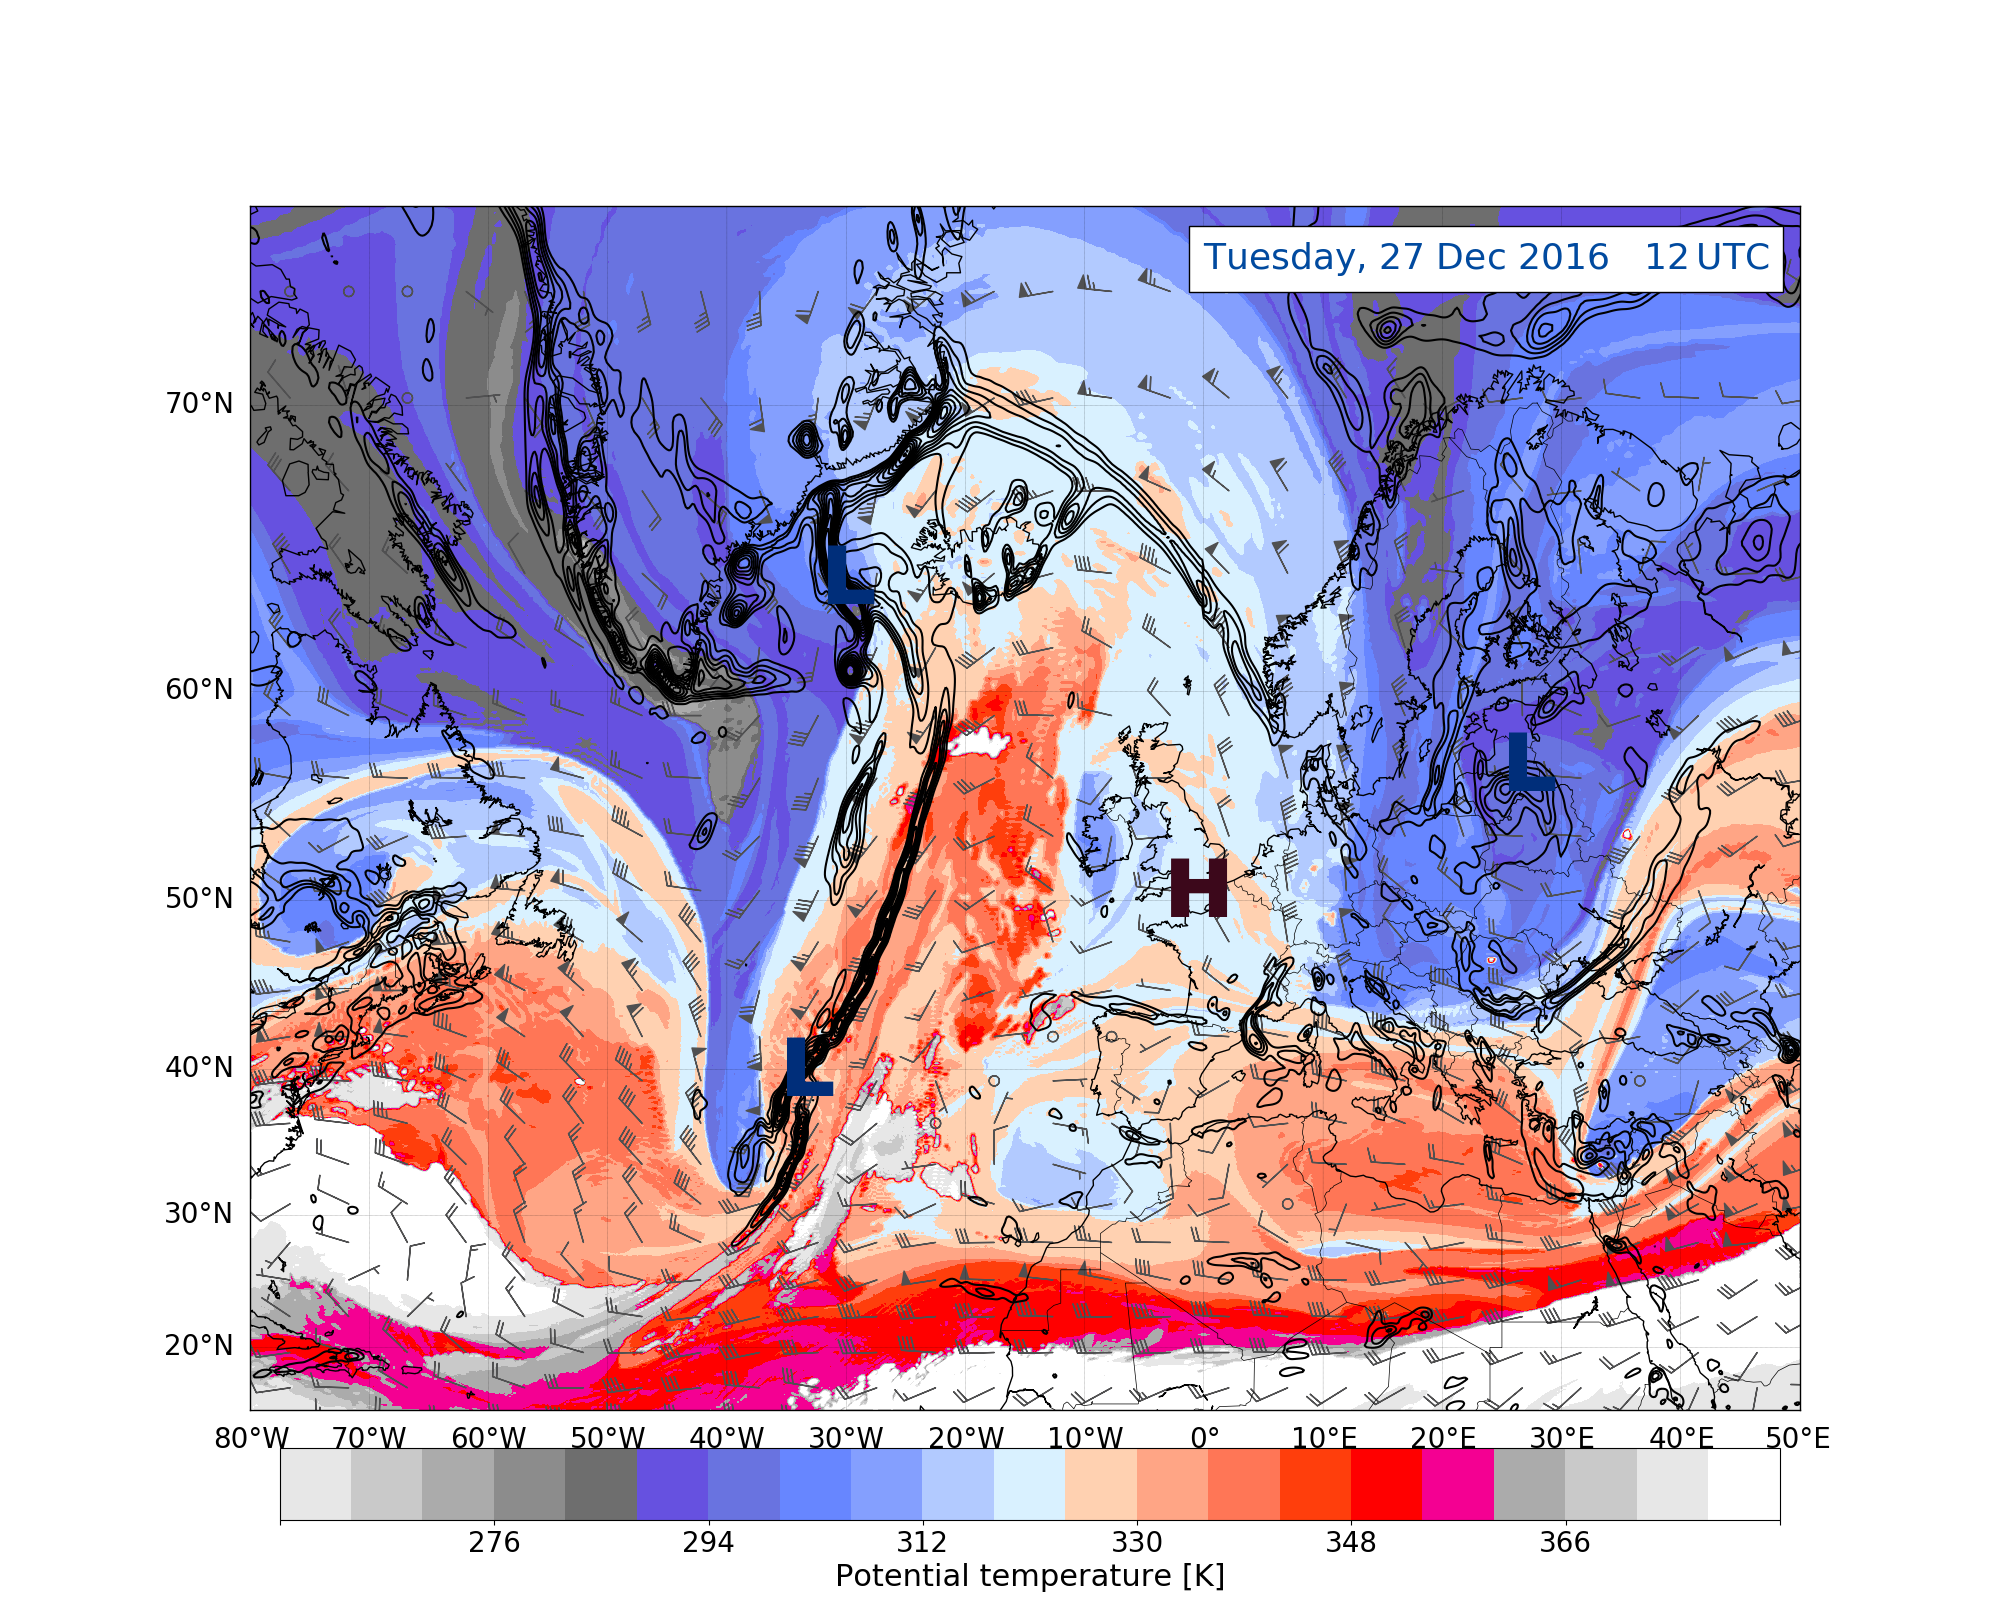
\includegraphics[trim={4.2cm 3.9cm 4.3cm 5.1cm},clip,
        width=\textwidth]{./fig_DynTropo/20161227_12}
        \caption{}\label{fig:DT27}
    \end{subfigure}   
%%%%%% label
    \begin{subfigure}[b]{\textwidth}
        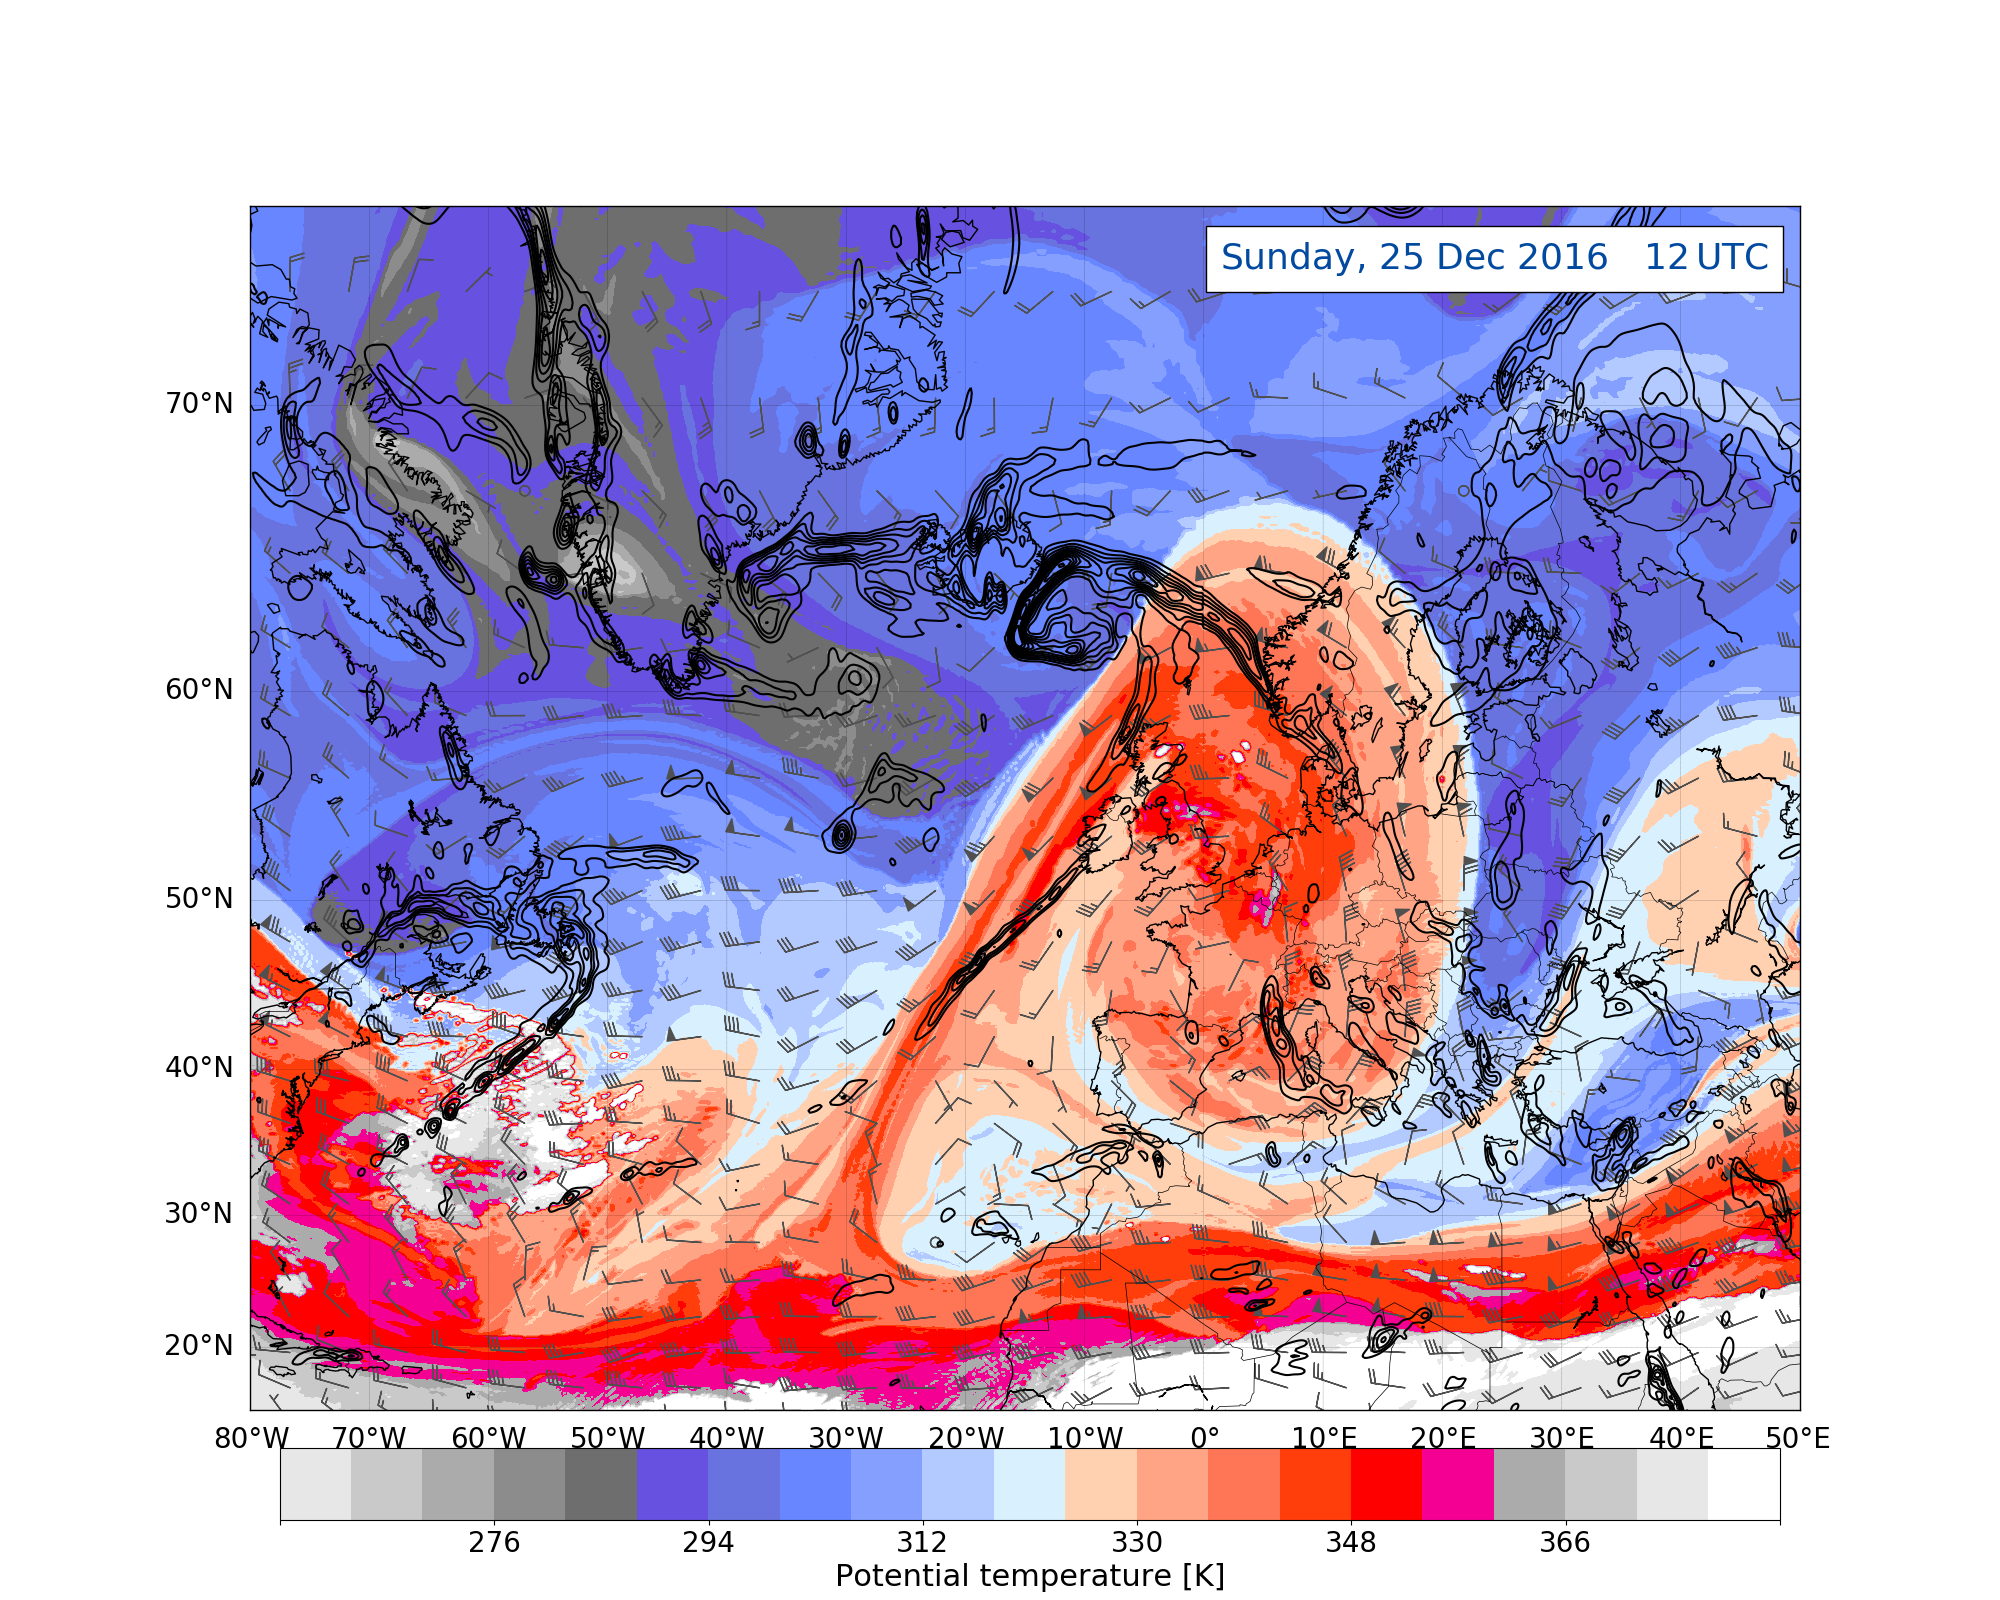
\includegraphics[trim={4.2cm 0cm 4.3cm 36.8cm},clip,
        width=\textwidth]{./fig_DynTropo/20161225_12}
    \end{subfigure}
    \caption{Dynamic tropopause analysis map, data from ECMWF at \SI{2}{PVU}. During \SIrange{20}{27}{\dec}. Potential temperature [K] at the \SI{2}{PVU} surface, shaded according to the colour bar. Total wind, barbs [\SI{}{\mPs}], and \SI{925}-\SI{850}{\hPa} layer-averaged surface relative vorticity (black contours, every \SI{.5e-4}{\per\second}).  }\label{fig:DynTropo}
\end{figure}
%%%%%%%%%%%%%%%%%%%%%%%%%%%%%%%%%%%%%%%%%%%%%%%%%%%%%%%%%%%%%%%%%%%%%%%%%%
